\section{Methods \label{sec:rank_lists_fusion}}

The idea of rank lists' fusion is to combine multiple rank lists in such a way that the resulting rank list produced is a more accurate modelling of a perfect rank list.
This perfect rank list contain every true links (same author document pairs) at the top and every false links (different author document pair) at the bottom, therefore maximizing every metrics in Section~\ref{sec:rl_eval}.

Two methods are proposed, one is based on the Z-Score normalization, and the second one use the logistic regression.

\subsection{Z-Score Fusion}

When merging rank lists, a problem arise: due to the difference of distance metric and/or text representation, the scores used in the rank list are of different order of magnitude.
Thus, simply applying the arithmetic mean on the scores for each rank list is not effective.

To mitigate this problem, a simple and rather effective approach is to normalize the scores of each rank lists independently using the Z-Score (See Definition~\ref{def:z_score} in Section~\ref{sec:normalization}).
Then one can compute a resulting score for each link as the arithmetic mean of scores in every Z-Score normalized rank lists.
The rank list can then be sorted by this new score.

Additionally, this method provide a framework for the fusion with both distance metrics and similarity metrics.
If distances and similarity score are encountered for a fusion, flipping the score sign for either the distance rank lists or similarity rank lists after the Z-Score normalization allow to fix these metrics differences.

This method can provide good results does not have any parameters, but lack theoretical foundations.

Example~\ref{ex:z_score_fusion} show an example for the Z-Score fusion computation using two simple rank lists.

\begin{example}
  \caption{Z-Score fusion of two rank lists}
  \label{ex:z_score_fusion}

  \begin{subexample}{\linewidth}
    \centering
    \subcaption{Rank list A (Mean = 50, Std = 40.82)}
    \begin{tabular}{c l r r}
      \toprule
      Rank & Link & Score & Z-Score \\
      \midrule
      1st & (0, 2) & $0$ & $-1.22$ \\
      2nd & (1, 2) & $50$ & $0$ \\
      3rd & (0, 1) & $100$ & $1.22$ \\
      \bottomrule
    \end{tabular}
  \end{subexample}

  \vspace{0.5cm}

  In this example, the scores does not satisfy the triangle inequality for the sake of simplicity.

  \vspace{0.5cm}

  \begin{subexample}{\linewidth}
    \centering
    \subcaption{Rank list B (Mean = 0.33, Std = 0.17)}
    \begin{tabular}{c l r r}
      \toprule
      Rank & Link & Score & Z-Score \\
      \midrule
      1st & (0, 2) & $0.1$ & $-1.37$ \\
      2nd & (0, 1) & $0.4$ & $0.39$ \\
      3rd & (1, 2) & $0.5$ & $0.98$ \\
      \bottomrule
    \end{tabular}
  \end{subexample}

  \vspace{0.5cm}

  \begin{subexample}{\linewidth}
    \centering
    \subcaption{Z-Score fusion}
    \begin{tabular}{c l r}
      \toprule
      Rank & Link & Mean Z-Score \\
      \midrule
      1st & (0, 2) & $(-1.22 + (-1.37)) / 2$ = $-1.30$ \\
      2nd & (1, 2) & $(0 + 0.98) / 2$ = $0.49$ \\
      3rd & (0, 1) & $(0.39 + 1.22) / 2$ = $0.81$ \\
      \bottomrule
    \end{tabular}
  \end{subexample}

\end{example}

\subsection{Regression Fusion \label{sec:regression_fusion}}

This second fusion method is based on logistic regression and is called regression fusion in this study.

Each rank list is ordered by a score, this score depends on the distance measure and text representation used, thus the order of magnitude across rank list can be different.
To avoid this problem, the second solution is to express the scores into a probability of being a true link.
To do so, the logistic regression is used.
This method is similar to the one proposed in \textit{Le Calvé and Savoy (2000)}'s paper~\cite{le_calve_database_merging} and was used for merging rank list issued from information retrieval systems.

The main idea here is to learn a logistic regression model for each combination of text representation and distance metrics (here denoted \textit{type of rank list}).
From each distinct rank list, features for each link are created.
We have selected the log of the relative rank and the link score.
Since a probability of being a true link is desired, the target value for each link is either 1 for the true links or 0 when it is a false link.
This feature construction is the same as the one used for the regression-based clustering method (ref. Section~\ref{sec:regression_based_clustering}).

One model per type of rank list is trained, this model can provide for any new same type rank list, probabilities for each link being of being a true link.

The probability framework can now be used on the rank list.
To obtain the most reliable probability given multiple observations (different rank lists), the regression fusion consists in computing the expected value for each link's probability using these observations.
In this case, the final value for sorting the rank list is an average of the probabilities, since no weighting is used on the rank lists.

The main advantage of this methodology is that it uses concrete statistical concepts.
But this technique has one main issue, that is the need of having examples to train the model.

\subsection{Veto}

The idea here is to provide a veto power for the rank lists, to try to improve the results.
The following assumption is made: if a link have a low probability in a rank list before the fusion.
This probably indicate a false link, thus having this link at the bottom of the rank list after the fusion can improve the results.

To fulfil the previously stated assumption, a possible way is to find every link in all rank lists before the fusion, where the probability is under a certain threshold.
Then we can alter their probabilities (probability of being a true link) with $-\infty$.
Every links below the probability threshold will have its final score also equal to $-\infty$ since the average with any number and $-\infty$ is always $-\infty$.
When sorting the rank list, the links with a resulting $-\infty$ score will subsequently be ranked at the bottom.
This veto method is also called $-\infty$-veto in this study.

Example~\ref{ex:veto_ninf} showcase an example when the veto can provide better results than the standard fusion in Example~\ref{ex:noveto}.
As you can see with the rank lists in the example, rank list 1 give a 0.20 probability for a link with ID = 4 of being a true link, but rank list 3 give this link a 0.80 probability.
The link with ID = 3 is ranked 3rd, but with the veto the link is ranked 5th.

One problem arise with this solution, multiple links can have a $-\infty$ probability.
The proposed solution is to set the probability of the affected links to one of these values instead: $0$, $-1$ or $-n$, with n equal to the number of rank lists to fuse.
The greater, the value, the stronger the penalty of the veto.
The $-\infty$ method is the only real veto, in the first meaning of the veto definition, the other methods can be considered as a weighted veto.

The $-n$, method provide a way to avoid having tie and keep the strong impact of the $-\infty$-veto when a lot of rank list are fused.
By setting to $0$, $-1$ or $-n$ can lighten the veto effect and conserve an order in the bottom rank links.
An example using the $0$-veto is presented in Example~\ref{ex:veto_0}.
Here the link with ID = 4 is ranked 4th due to a lighter effect of this veto.
Link with ID = 5 is still rank at the bottom.

\begin{example}
  \centering
  \caption{Fusion without veto}
  \label{ex:noveto}

  \begin{subexample}{\linewidth}
    \centering
    \subcaption{Rank lists}
    \resizebox{\linewidth}{!}{
    \begin{tabular}{c c|c c|c c}
      \toprule
      \multicolumn{2}{c}{Rank list 1} &
      \multicolumn{2}{c}{Rank list 2} &
      \multicolumn{2}{c}{Rank list 3} \\
      Link ID & Score &
      Link ID & Score &
      Link ID & Score \\
      \midrule
      0 & 0.95 & 0 & 0.90 & 5 & 0.90 \\
      1 & 0.75 & 3 & 0.70 & 4 & 0.80 \\
      2 & 0.60 & 4 & 0.65 & 0 & 0.70 \\
      3 & 0.50 & 1 & 0.50 & 1 & 0.60 \\
      4 & 0.20 & 2 & 0.30 & 2 & 0.50 \\
      5 & 0.10 & 5 & 0.10 & 3 & 0.40 \\
      \bottomrule
    \end{tabular}
    }
  \end{subexample}

  \vspace{0.5cm}

  \begin{subexample}{\linewidth}
    \centering
    \subcaption{Rank lists' fusion}
    \resizebox{\linewidth}{!}{
    \begin{tabular}{l l l}
      \toprule
      Rank & Link ID & Average \\
      \midrule
      1st & 0 & $(0.95 + 0.90 + 0.70)/3 = 0.85$ \\
      2nd & 1 & $(0.75 + 0.50 + 0.60)/3 = 0.62$ \\
      3rd & 4 & $(0.20 + 0.65 + 0.80)/3 = 0.55$ \\
      4th & 3 & $(0.50 + 0.70 + 0.40)/3 = 0.53$ \\
      5th & 2 & $(0.60 + 0.30 + 0.50)/3 = 0.47$ \\
      6th & 5 & $(0.10 + 0.10 + 0.90)/3 = 0.37$ \\
      \bottomrule
    \end{tabular}
    }
  \end{subexample}
\end{example}

\begin{example}
  \centering
  \caption{Fusion with $-\infty$-veto at 0.25}
  \label{ex:veto_ninf}

  \begin{subexample}{\linewidth}
    \centering
    \subcaption{Rank lists}
    \resizebox{\linewidth}{!}{
    \begin{tabular}{c c|c c|c c}
      \toprule
      \multicolumn{2}{c}{Rank list 1} &
      \multicolumn{2}{c}{Rank list 2} &
      \multicolumn{2}{c}{Rank list 3} \\
      Link ID & Score &
      Link ID & Score &
      Link ID & Score \\
      \midrule
      0 & 0.95 & 0 & 0.90 & 5 & 0.90 \\
      1 & 0.75 & 3 & 0.70 & 4 & 0.80 \\
      2 & 0.60 & 4 & 0.65 & 0 & 0.70 \\
      3 & 0.50 & 1 & 0.50 & 1 & 0.60 \\
      4 & -inf & 2 & 0.30 & 2 & 0.50 \\
      5 & -inf & 5 & -inf & 3 & 0.40 \\
      \bottomrule
    \end{tabular}
    }
  \end{subexample}

  \vspace{0.5cm}

  \begin{subexample}{\linewidth}
    \centering
    \subcaption{Rank lists' fusion}
    \resizebox{\linewidth}{!}{
    \begin{tabular}{l l l}
      \toprule
      Rank & Link ID & Average \\
      \midrule
      1st & 0 & $(0.95 + 0.90 + 0.70)/3 = 0.85$ \\
      2nd & 1 & $(0.75 + 0.50 + 0.60)/3 = 0.62$ \\
      3rd & 3 & $(0.50 + 0.70 + 0.40)/3 = 0.53$ \\
      4th & 2 & $(0.60 + 0.30 + 0.50)/3 = 0.47$ \\
      5-6th & 4 & $(-\infty + 0.65 + 0.80)/3 = -\infty$ \\
      5-6th & 5 & $(-\infty + -\infty + 0.90)/3 = -\infty$ \\
      \bottomrule
    \end{tabular}
    }
  \end{subexample}
\end{example}

\begin{example}
  \centering
  \caption{Fusion with $0$-veto at 0.25}
  \label{ex:veto_0}

  \begin{subexample}{\linewidth}
    \centering
    \subcaption{Rank lists}
    \resizebox{\linewidth}{!}{
    \begin{tabular}{c c|c c|c c}
      \toprule
      \multicolumn{2}{c}{Rank list 1} &
      \multicolumn{2}{c}{Rank list 2} &
      \multicolumn{2}{c}{Rank list 3} \\
      Link ID & Score &
      Link ID & Score &
      Link ID & Score \\
      \midrule
      0 & 0.95 & 0 & 0.90 & 5 & 0.90 \\
      1 & 0.75 & 3 & 0.70 & 4 & 0.80 \\
      2 & 0.60 & 4 & 0.65 & 0 & 0.70 \\
      3 & 0.50 & 1 & 0.50 & 1 & 0.60 \\
      4 & 0.00 & 2 & 0.30 & 2 & 0.50 \\
      5 & 0.00 & 5 & 0.00 & 3 & 0.40 \\
      \bottomrule
    \end{tabular}
    }
  \end{subexample}

  \vspace{0.5cm}

  \begin{subexample}{\linewidth}
    \centering
    \subcaption{Rank lists' fusion}
    \resizebox{\linewidth}{!}{
    \begin{tabular}{l l l}
      \toprule
      Rank & Link ID & Average \\
      \midrule
      1st & 0 & $(0.95 + 0.90 + 0.70)/3 = 0.85$ \\
      2nd & 1 & $(0.75 + 0.50 + 0.60)/3 = 0.62$ \\
      3rd & 3 & $(0.50 + 0.70 + 0.40)/3 = 0.53$ \\
      4th & 4 & $(0.00 + 0.65 + 0.80)/3 = 0.48$ \\
      5th & 2 & $(0.60 + 0.30 + 0.50)/3 = 0.47$ \\
      6th & 5 & $(0.00 + 0.00 + 0.90)/3 = 0.30$ \\
      \bottomrule
    \end{tabular}
    }
  \end{subexample}
\end{example}

\subsection{Soft-veto}

As an extension to the veto method, an additional desired constraint is to favor top ranked link and as well as penalizing bottom ranked links.
This constraint can be easily explained by observing the distribution of the distances according to the rank.
Figure~\ref{fig:distance_over_rank} clearly show us the top ranks and bottom ranks have a sharper difference in distance than in than the middle section.

Top ranks correspond to documents with the same author, and bottom links correspond to documents with different authors.
Assuming that the top ranks are true links after the rank lists' fusion, these links should also appear top rank.
The same reasoning can be applied for the bottom links by assuming them as false links.
A weighting curve, here called soft-veto, can be design accordingly such that the score of top links are boosted, and bottom links score hindered.

Using the inverse of the sigmoid function, such a curve can be modelled.
Definition~\ref{def:sigmoid} show the sigmoid function and its inverse function.

\begin{definition}[Sigmoid and Sigmoid inverse function \label{def:sigmoid}]
  Sigmoid:
  \begin{gather*}
    S(x) = \frac{1}{1+e^{-x}}
  \end{gather*}

  Sigmoid inverse:
  \begin{gather*}
    S^{-1}(x) = -\ln{\frac{x-1}{x}}
  \end{gather*}
\end{definition}

Since the inverse of the sigmoid function is continuous and the number of links in a rank list is discrete, the idea is to sample values in this curve at regular intervals.

Controlling the steepness of this curve can influence the strength of the veto.
To control the steepness, a parameter called $c$ is introduced.
$c$ correspond to a position on the x-axis of the sigmoid function.
The sampling of the sigmoid inverse is done in the interval $\left[S(c), S(c)\right]$.
A large interval gives a greater steepness and a small interval a less steep curve.
$c$ can not be equal to 0 otherwise the interval is a single number (often called degenerate interval).
The $c$ parameter must be in the interval $\left]0, \infty\right[$.
With a value close to $0$, the soft-veto have a weak effect.
With a large value, for example 20, the soft veto has a strong effect on the top and bottom, see Figure~\ref{fig:s_curve_c}.

To break the curve symmetry and to be able to increase the conservation of the top rank while decreasing the conservation of the bottom ranked.
The solution proposed is to have a new parameter $r$.
$r \cdot N$ samples are taken for the left side of the curve $\left[S(-c), S(0)\right]$
And $(1-r) \cdot N$ samples for the right side of the curve $\left[S(0), S(c)\right]$.
Figure~\ref{fig:s_curve_r} shows the $r$ parameter influence on a sigmoid with $c = 4$ and $r \in \left[0.1, 0.9\right]$.
The $r$ parameter must be in the interval $\left]0, 1\right[$.
With a value close to $0$ the soft-veto have a strong effect on the top ranked links.
With a large value, a strong effect on the bottom ranked links, see Figure~\ref{fig:s_curve_r}.

To apply the soft-veto, each score in the rank list is multiplied by the curve at the corresponding rank.
This soft-veto methodology aimed to be used on rank list before fusing, to have a more cleaved decision on the links positions.
This strategy can be use on any type of scoring method (similarity, distances, Z-Score scores or probabilities).

\begin{figure}
  \centering
  \caption{Distance values over rank in the rank list using the smoothed Manhattan distance, $500$-MF tokens on the Brunet dataset}
  \label{fig:distance_over_rank}
  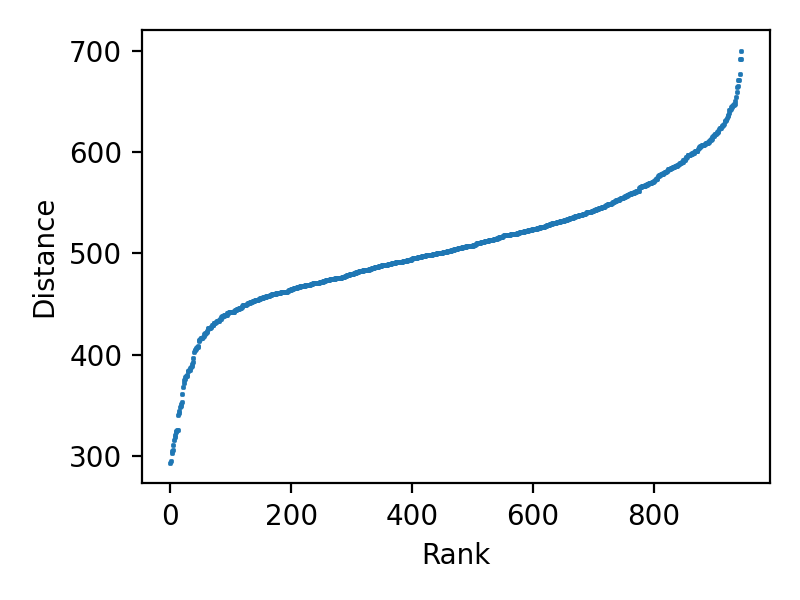
\includegraphics[width=\linewidth]{img/distance_over_rank.png}
\end{figure}

\begin{figure}
  \centering
  \caption{Curve parameters}
  \label{fig:s_curve_params}

  \subcaption{$S^-1(x)$, 1000 samples (for a rank list with 1000 links) in $\left[S(-c), S(+c)\right]$}
  \label{fig:s_curve_c}
  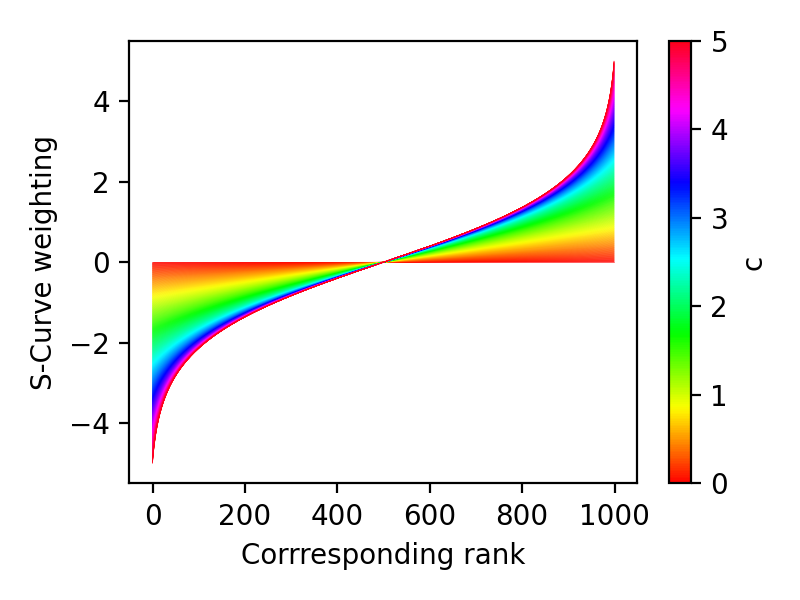
\includegraphics[width=\linewidth]{img/s_curve_c.png}

  \vspace{0.5cm}

  \subcaption{1000 sample of $S^-1(x)$ with $r \cdot N$ samples for $\left[S(-c), S(0)\right]$ and $(1-r) \cdot N$ samples for $\left[S(0), S(c)\right]$}
  \label{fig:s_curve_r}
  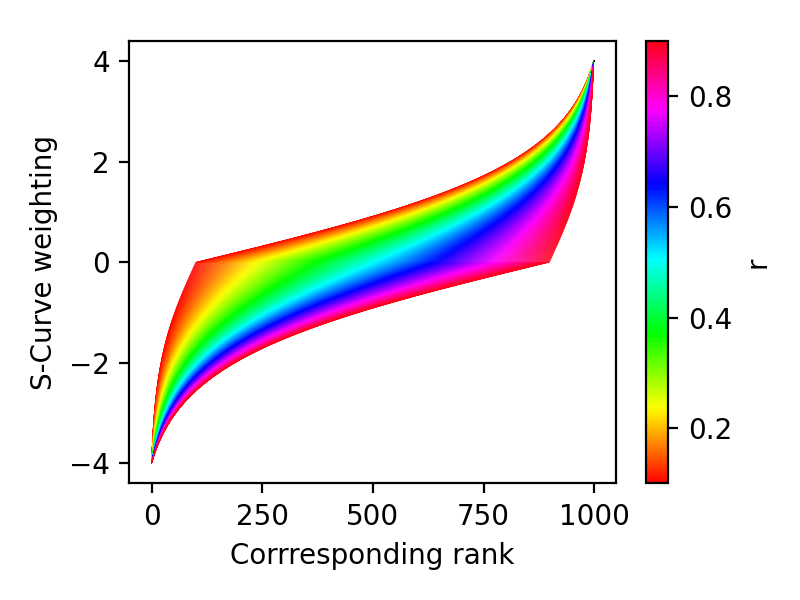
\includegraphics[width=\linewidth]{img/s_curve_r.png}

  \vspace{0.5cm}

  \subcaption{Example of a curve with $c=4$ and $r=0.85$}
  \label{fig:s_curve_example}
  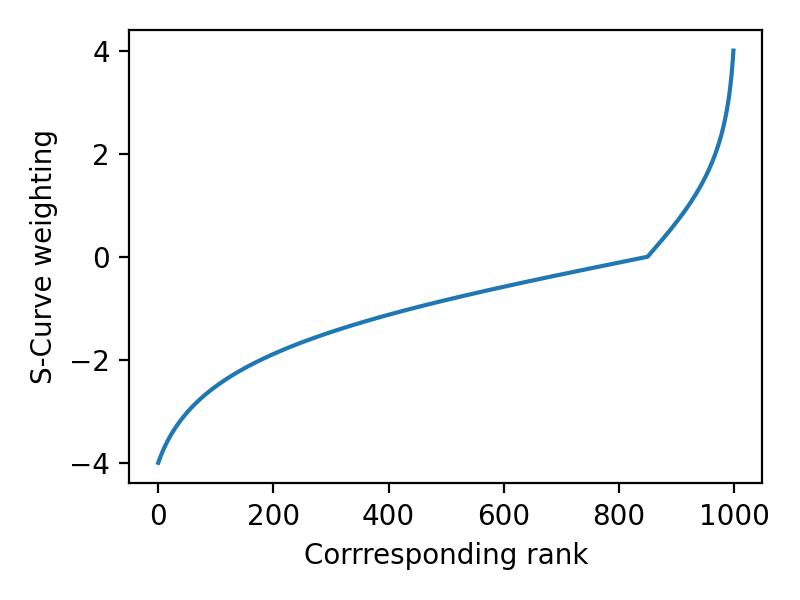
\includegraphics[width=0.9\linewidth]{img/s_curve_example.png}
\end{figure}
